\chapter{Desenvolvimento}
\label{cap:desenvolvimento}
%
%\section{Implementação da biblioteca}
%
%
A \textit{SAGA Game Library} é uma \textit{engine} orientada a objeto desenvolvida em C++ sobre a API Allegro 5. Ela possui suporte a diversos formatos de arquivos de imagem (PNG, JPEG e GIF, por exemplo), a criação de cenários usando o editor de níveis Tiled, suporte ao uso de fontes de texto TTF e a reprodução de diversos formatos de arquivos de áudio. Também possui gerenciamento automático de recursos (imagem, fontes e áudio), o que possibilita economia significativa de memória. A biblioteca fornece uma estrutura para implementação do \textit{game loop} e suporte para eventos de teclado, \textit{mouse} e \textit{joystick} também estão presentes. 
\par 
Após a fase de projeto, deu-se sequência à fase de implementação do mesmo, de modo a torná-lo orientado a objetos. Internamente, a \textit{SAGA Game Library} consiste em um \textit{package} denominado \textit{sgl} e subdivididas em 4 outros \textit{packages} com funções específicas: \textit{image, font, audio e input}.
%
%
\begin{itemize}
 \item image: consiste nas classes exclusivamente relacionadas à parte gráfica da \textit{engine}, o que inclui manipulação de arquivos de imagens e carregamento e renderização de cenários do jogo;
 \item font: é o responsável pela parte textual da biblioteca. Ele carrega uma fonte no formato TTF (``True Type Font'') padrão do Windows e a utiliza para escrever textos na tela de jogo;
 \item audio: \textit{package} destinado ao carregamento, manuseio e reprodução dos arquivos de áudio;
 \item input: inclui todas as funções relacionadas aos comandos recebidos pelos dispositivos de entradas do computador (teclado, \textit{mouse} e \textit{joystick}).
\end{itemize}
%
\par
Na Figura \ref{pacotes} é possível visualizar o esquema da organização da \textit{engine}. A seguir, serão abordados os principais recursos da biblioteca bem como os detalhes da suas respectivas implementações.
%
%
%
%
\begin{figure}[H]
    \centering
     \caption{Esquema estrutural da SGL. }
    \label{pacotes}
    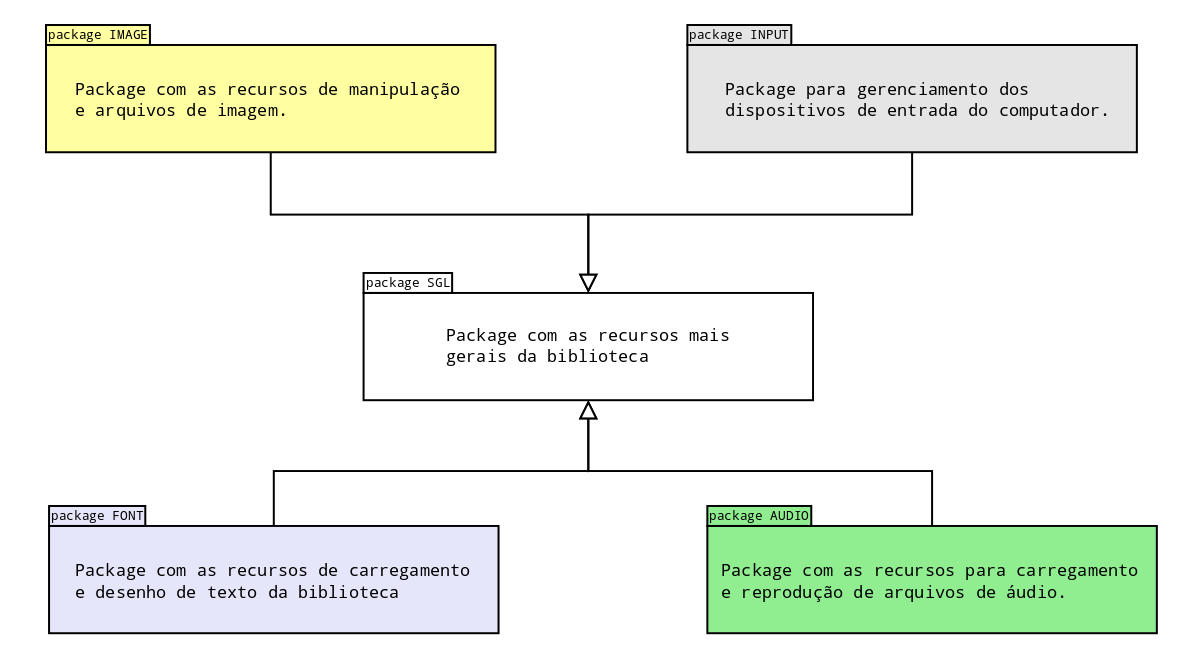
\includegraphics[scale = 0.2]{Imagens/pacotes.png}
    \\Fonte: Elaborada pelos autores.
\end{figure}
%
%
%
\section{SGL}
%
%
É o pacote mais geral e que engloba todos os outros. Quando a funcionalidade de uma classe não é específica ou é usada como ferramenta auxiliar em outras classes, ela é colocada nesse pacote.
%
%============================================
\subsection{AllegroStarter}
%
Cada um dos módulos da Allegro deve ser inicializado antes de seu uso. A classe AllegroStarter é responsável por alocar e também por desalocar os recursos da Allegro quando o programa é fechado. Uma exceção é lançada caso algum dispositivo apresente problemas durante a inicialização. Também contém informações sobre a atual versão da Allegro. 
%
%
%============================================
\subsection{SGLException}
%
É a classe que captura e trata as exceções que possam ocorrer durante a execução do programa, como inicialização dos componentes da Allegro e carregamento de arquivos de imagem, fonte e áudio. A classe é uma especialização de \texttt{std::exception}. O código a seguir exemplifica o uso desta classe.
%
\lstinputlisting{CodigoFonte/ExemploSGLException.cpp}
%
\par 
Caso ocorra algum erro de inicialização da Allegro, a função \textit{al\_init()} retornará \textit{false}, fazendo com que o programa execute o conteúdo do \textit{if} e lance a exceção. No console, teremos a mensagem:  ``\textit{terminate called after throwing an instance of `sgl::Exception'
what(): Failed to initialize ALLEGRO\_Lib.}''.
%
%
%============================================
\subsection{Color}
%
%
A classe Color possui recursos para se trabalhar com diversos formatos de especificação de cores, como RGB e formato hexadecimal utilizado em HTML. Os objetos dessa classe podem ser usadas, por exemplo, para colorir a tela ou alterar a cor de uma determinada fonte de texto. Ela aceita dois construtores. Com o primeiro deles é possível definir cores no formato RGB. Para isso, o construtor recebe três parâmetros que variam de 0 a 255, um para vermelho, outro para verde e outro para azul, respectivamente. O segundo construtor aceita \textit{strings} no formato hexadecimal utilizado em HTML ou o nome em inglês de uma cor, desde que ele já esteja predefinido. Alguns dos nomes válidos são: \textit{cyan}, \textit{lightgreen}, \textit{green}, entre outros. Caso o nome de uma cor inexistente seja passado como parâmetro, o construtor cria um objeto com as coordenadas RGB iguais a 0 (cor preta). A seguir temos alguns exemplos de uso da classe Color.
%
%
\lstinputlisting{CodigoFonte/ExemploColor.cpp}
%
%
%============================================
\subsection{Video}
%
%
A classe Video é responsável por gerenciar todos os recursos de vídeo da \textit{engine}. Através dela, tem-se acesso a todas as rotinas pertinentes (de atualização de tela, posicionamento, e outros eventos) para o gerenciamento de vídeo. A classe também possibilita a escolha por parte do usuário de criar um \textit{display} no formato de janela ou em tela cheia (\textit{fullscreen}).
%, e também permite a escolha de uma API para renderização 3D, como OpenGL (Linux e Windows) e DirectX (Windows). 
\par 
Quando criarmos um objeto da classe Video, devemos definir as dimensões do janela ou \textit{display}, passando como parâmetro a largura e altura desejadas e o modo (WINDOWED, FULLSCREEN) no construtor da classe. Por padrão, a cor de fundo do vídeo é preta, podendo ser alterada. Também existe a possibilidade de adicionar um ícone e um título para a janela. A função \textit{refresh()} é responsável por por transferir o conteúdo da memória de vídeo para o \textit{display} e deve ser chamada sempre que seja necessário atualizar o \textit{display}, caso contrário, nenhum das ações realizadas pelas rotinas de desenho serão visualizadas. 
\par 
A principal dificuldade na implementação dessa classe foi aprender como a Allegro fazia uso da memória de vídeo e entender conceitos como o taxa de atualização do \textit{display}. Outro fator preocupante diz respeito ao desempenho da renderização da \textit{display}, que foi resolvido ajustando a Allegro para que ela armazenasse todas as imagens a serem desenhadas na memória de vídeo ao invés da memória RAM. Essa configuração apresentou resultados significativos no uso do processador uma vez que enquanto as imagens armazenadas na RAM utilizavam 25\% da CPU, as mesmas imagens armazenadas na memória de vídeo não consumiam mais de 2\% do processador durante o processo de desenho no \textit{display}.
\par
A Figura \ref{umlVideo} mostra a classe Video em detalhes.
%
%
%
%
\begin{figure}[H]
    \centering
    \caption{UML da classe Video.}
    \label{umlVideo}
    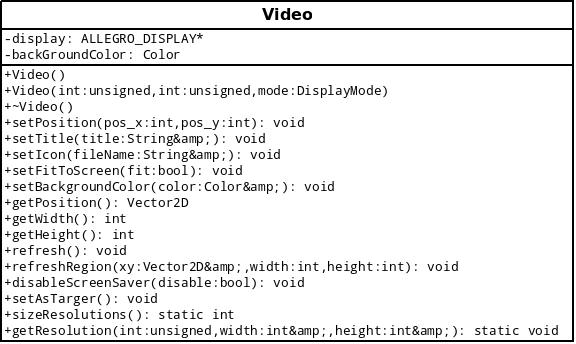
\includegraphics[scale = 0.5]{uml/video.jpeg}
    \\Fonte: Elaborada pelos autores.
\end{figure}
%
%
e a Figura \ref{display}, um exemplo de uso da mesma.
%
%
\lstinputlisting{CodigoFonte/ExemploDisplay.cpp}
%
%
\begin{figure}[H]
    \centering
    \caption{\textit{Display} criado com o uso da classe Video.}
    \label{display}
    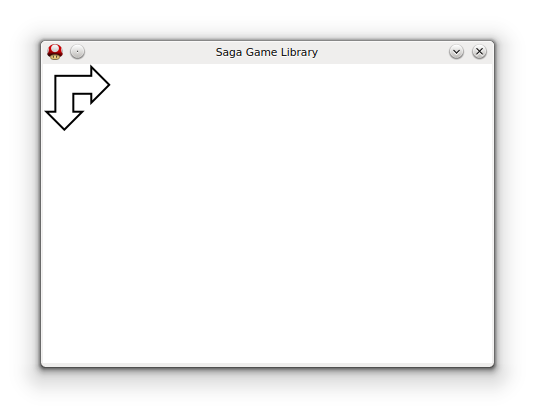
\includegraphics[scale = 0.40]{Imagens/display.png}
    \\Fonte: Elaborada pelos autores.
\end{figure}
%
%
%============================================
\subsection{Vector2D}
%
%
A classe Vector2D, tal qual o nome diz, define um vetor bidimensional, iniciando-se no ponto (0,0) da tela e indo até o ponto (x,y) definido pelo usuário, sendo responsável pelo posicionamento de qualquer entidade, seja ela um imagem ou um texto, no \textit{display}. A escolha do uso de vetores ao invés de simples coordenadas deve-se a vantagens como simplicidade e padronização. Muitas operações matemáticas, como deslocamento, rotações e escalonamentos, são feitas utilizando vetores. Até mesmo efeitos de física, como gravidade e aceleração, são executados usando como base os conceitos da mecânica clássica. A vantagem do vetor sobre um par de coordenadas (x,y) deve-se à quantidade de informação que o primeiro carrega. Enquanto um ponto representa apenas uma localização no espaço, um vetor possui uma direção, sentido e magnitude. 
\par 
Assim como ocorre na geometria, os vetores também possibilitam diversas operações algébricas entre eles, através da sobrecarga de operadores. Soma e subtração de vetores e normalização são algumas das operações possíveis e que podem ser usadas para se obter interessantes resultados, como a simulação de gravidade, ilustrada na figura \ref{VetorGravidade}, onde temos um vetor representando o deslocamento do personagem e outro representando a força gravitacional.
%
%
%
\begin{figure}[H]
    \centering
    \caption{Uso de vetores na simulação de gravidade.}
    \label{VetorGravidade}
    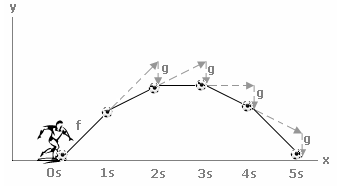
\includegraphics[scale = 0.8]{Imagens/VetorGravidade.png}
    \\Fonte: Imagem retirada de \cite{PontoV};
\end{figure}
%
%
A seguir temos um exemplo com algumas das operações de Vector2D.
%
\lstinputlisting{CodigoFonte/ExemploVector2D.cpp}
%
%
%============================================
\subsection{BoundingBox}
%
%
Esta classe cria um retângulo usando dois objetos Vector2D. Ela possui rotinas para alterar a posição do retângulo e também verificar se houve colisão com outro retângulo. A BoundingBox é utilizada na biblioteca como um mecanismo para detectar se ocorreu colisão entre duas entidades, como por exemplo, um personagem e um objeto do cenário, como uma parede. Se ocorreu a colisão, o método responsável pela verificação retorna \textit{true}, caso contrário ele retorna \textit{false}. Vale ressaltar que a classe é responsável apenas por verificar se ocorreu ou não colisão, sendo de responsabilidade do usuário o tratamento adequado dessa colisão.
%
%
%============================================
\subsection{Geometrics}
%
%
Geometrics é a classe usada para desenhar primitivas geométricas tendo como atributos um inteiro para armazenar a espessura da linha e duas variáveis da classe Color, uma para cor da linha e outra para cor do preenchimento. O construtor padrão inicializa a espessura com 1, a cor de preenchimento como branca e a cor da linha como preta. Outro construtor da ao usuário a liberdade de definir os valores como quiser. Através da classe Geometrics é possível desenhar linhas, triângulos, retângulos, retângulos com cantor arredondados, elipses, círculos e arcos. 
\par 
Exemplos: 
\par
Declaração de vetores que serão usados:
%
\begin{lstlisting}
  Vector2D a(200,150);
  Vector2D b(280,150);
  Vector2D c(350,150);
  Vector2D d(200,100);
\end{lstlisting}
%
%
\par 
No construtor da classe, dizemos que a espessura da linha é 5 e que sua cor é verde. O terceiro parâmetro diz respeito à cor de preenchimento da forma geométrica a ser desenhada. 
%
\begin{lstlisting}
 Geometrics geo(5, Color("green"), Color("purple"));
\end{lstlisting}
%
Em \textit{drawCircle()}, o primeiro parâmetro deve ser a posição do círculo. O segundo é o raio e o terceiro é do tipo booleano. Se for \textit{true}, o objeto será preenchido com a cor definida no construtor. Se for \textit{false}, a forma não terá preenchimento algum. Note que parte do círculo não aparece porque está atrás do triângulo. Se o triângulo não tivesse cor de preenchimento, essa parte estaria visível. 
%
\begin{lstlisting}
 geo.drawCircle(a, 100, false);
 geo.drawTriangle(b, c, d, true);
\end{lstlisting}
% 
%
O resultado pode ser visualizado na Figura \ref{ExemploGeometric}.
%
\begin{figure}[H]
    \centering
    \caption{Exemplo de uso da classe Geometrics.}
    \label{ExemploGeometric}
    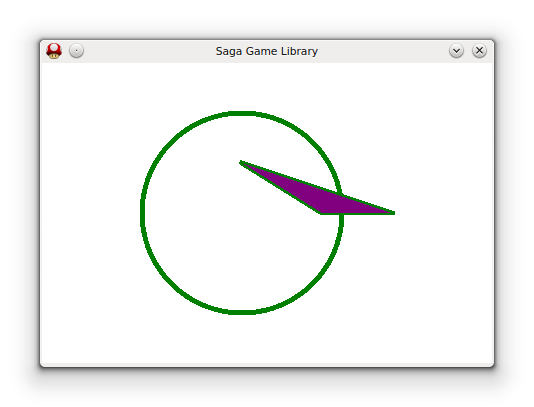
\includegraphics[scale = 0.7]{Imagens/ExemploGeometric.png}
    \\Fonte: Elaborada pelos autores.
\end{figure}
%
%
%===========================================
\subsection{TimeHandler}
%
%
TimeHandler é a classe que possui rotinas relacionadas à contagem de tempo, em milissegundos. A contagem de tempo é algo muito importante no desenvolvimento de \textit{games}, pois ela pode ser usada para controlar a contagem de atualizações por segundo do \textit{display} ou até mesmo executar ações do jogo que são dependentes do tempo. A Allegro possui suas próprias rotinas de contagem de tempo e a classe TimeHandler encapsula essas rotinas de modo a facilitar sua utilização, permitindo iniciar, pausar, retornar uma
contagem de tempo e encerrá-la.
\par
O trecho a seguir faz a contagem de tempo necessária para o computador percorrer a extensão de um tipo \textit{unsigned int} em arquitetura 32 bits.
%
\begin{lstlisting}
  TimeHandler time;
  time.start();
  for (unsigned int i = 0; i<4294967295; i++){} 
  time.pause();
  float t = time.getTicks();
\end{lstlisting}
%
\par 
A execução do código acima nos devolve a seguinte saída (em segundos): 
%
\begin{lstlisting}
  t = 17.0142
\end{lstlisting}
%
%===========================================
\subsection{Resource e ResourceManager}
%
A classe Resource (Figura \ref{ResourceManager}) representa um recurso (áudio, imagem ou fonte) a ser utilizada no jogo e é uma classe abstrata que serve de base para as classes ImageResource, usada para o carregamento de imagens, FontResource utilizada no carregamento de fontes \textit{True Type}, AudioStreamResource e AudioSampleResource, que representam \textit{samples} e \textit{streams} de áudio. Quando um arquivo é carregado, seja ele fonte \textit{True Type}, imagem ou áudio, o mesmo é armazenado em sua respectiva classe filha de Resource. Deste modo conseguimos separar de maneira clara cada tipo de recurso, sendo que cada classe filha possui métodos para alocação e desalocação desse recursos pela Allegro além de métodos próprios para se trabalhar com o seu tipo de recurso. 
%
\par
Arquivos como imagens e áudio, podem ocupar tamanho razoável na memória (RAM e ROM) e apresentar um custo computacional considerável quando são carregados. No desenvolvimento de \textit{softwares}, buscar o máximo em economia de memória e desempenho é um aspecto importante. Porém, quando o \textit{software} em questão é um jogo eletrônico, esse aspecto passa a ser algo essencial. Jogos eletrônicos contam com rotinas para simulação de física, de inteligência artificial, de renderização e de carregamento de recursos são rotinas que demandam muito processamento. Além disso, tem-se os recursos que devem ser alocados, como arquivos de imagem e áudio, por exemplo. Com o objetivo de ter uma economia de memória e processamento, nota-se que o carregamento de um mesmo recurso várias vezes torna-se um inconveniente, conforme será explicado posteriormente. A classe ResourceManager foi criada para corrigir esse problema.
%
%
\begin{figure}[h]
    \centering
    \caption{UML detalhando as classes Resource e ResourceManager.}
    \label{ResourceManager}
    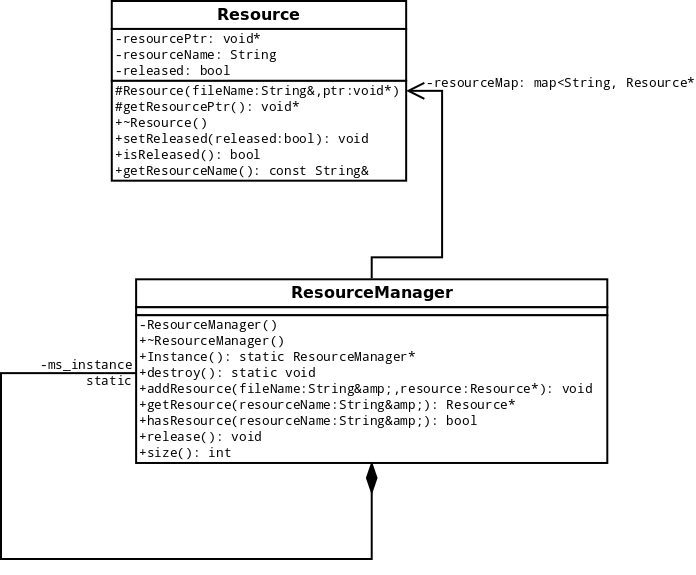
\includegraphics[scale = 0.4]{uml/ResourceManager.png}
    \\Fonte: Elaborada pelos autores.
\end{figure}
%
%
\par 
A ResourceManager (Figura \ref{ResourceManager}) é a classe responsável por executar esse gerenciamento de recursos. Ela possui como principal atributo um objeto da classe \textit{map} da biblioteca STL, chamado \textit{resourceMap}, que usa como chave para armazenamento os \textit{paths} dos recursos carregados.
\par
Esta estrutura permite o gerenciamento dos recursos de forma otimizada, fazendo que haja economia de memória e processamento. É muito mais rápido para o programa apenas reproduzir um recurso já carregado do que ter de carregá-lo novamente. É muito importante ter esse tipo de gerenciamento, especialmente para jogos com imagens muito repetitivas. O algoritmo usado pelas classes que fazem uso do ResourceManager é o seguinte: procura-se pelo objeto (pertencente a uma das classes filhas de Resource), utilizando o nome do seu arquivo, no mapa de Resources na ResourceManager. Se o mesmo for encontrado, a ResourceManager retorna um ponteiro desse objeto, caso contrário criamos esse novo Resource e o inserimos no mapa de Resources. A seguir podemos verificar o uso desse algoritmo no método que faz o carregamento das imagens na biblioteca. O padrão \textit{Singleton} foi utilizado devido a classe exercer uma papel de gerenciamento, ou seja, ter mais de uma classe gerenciando os recursos criados apenas tornaria mais custosa a utilização da mesma, uma vez que teríamos de procurar do resourceMap de cada ResourceManager pelo objeto Resource desejado.
%
\lstinputlisting{CodigoFonte/ExemploImageResouce.cpp}
%
\par 
Nesses casos a diferença entre ter ou não ter esse gerenciamento de recursos é grande e pode influenciar na performance do jogo, como podemos ver no exemplo a seguir.
\par 
De modo a verificar as vantagens do uso da ResourceManager, executamos o seguinte código e realizamos algumas medições: 
%
%
\begin{lstlisting}

  // Vetor contendo a imagem para o nosso jogo
  ALLEGRO_BITMAP* v_imagens[5000];
      
  // Carregamos cada uma das ALLEGRO_BITMAP
  for( int i=0; i < 5000; i++ )
  {
       v_imagens[i] = al_load_bitmap("sprite.png");
  }
  
\end{lstlisting}
%
\par
Esse código faz a Allegro carregar um conjunto de 5000 ALLEGRO\_BITMAPs, todas com a mesma imagem. Isso consumiu cerca de 471 MB de memória e exigiu 25\% do processador, levando 4,136 segundos para realizar carregamento das imagens. 
\par 
O código a seguir executa o mesmo algoritmo de antes, porem realiza a alocação de 5000 objetos do tipo ImageResource (carregando o mesmo arquivo de imagem). A classe ImageResource é a classe filha de Resource responsável pelo carregamento e desalocação dos arquivos de imagens. 
%
%
\begin{lstlisting}

  // Vetor contendo a imagem para o nosso jogo
  ImageResource* v_imagens[5000];
	
  // Carregamos cada uma das ImageResource
  for( int i=0; i < 5000; i++ )
  {
      v_imagens[i] = ImageResource::loadImageResource("sprite.png");
  }
	      
\end{lstlisting}
%
\par 
Após a execução do algoritmo, constatamos que a memória ocupada foi aproximadamente 1,912 KB (0,39\% da memória alocada anteriormente) e que a rotina consumiu apenas 2\% de processamento, levando aproximadamente 0,0264 segundos (0,638\% do tempo anterior) para realizar o carregamento. Com esse teste, ficam claras as vantagens de uso da \textit{SAGA Game Library}, ao invés de utilizar somente a ALLEGRO. Esses valores podem ser visualizados na Tabela \ref{tabelaEconomia}.
%
% 
\begin{table}[H]
\centering
\caption{Comparação de desempenho entre Allegro e SAGA Game Library.}
\begin{tabular}{|c|c|c|}\hline
\textbf{Parâmetro Analisado} & \textbf{Allegro} & \textbf{SAGA Game Library}\\\hline
\textbf{Memória utilizada} & 471 MB & 1,912 KB\\\hline
\textbf{Uso do processador} & 25\% & 2\% \\\hline
\textbf{Tempo de carregamento} & 4,136 seg. & 0,0264 seg.\\\hline
\end{tabular}
\\Fonte: Dados obtidos em simulações realizadas pelos alunos.
\label{tabelaEconomia}
\end{table}
%
%
\par
A maior dificuldade encontrada na implementação da ResourceManager foi implementar a desalocação dos \textit{resources} criados. Inicialmente implementamos um contador de referências, de forma que, quando um objeto Resource não fosse mais utilizado por nenhum outro objeto, ele seria removido do mapa de \textit{resources}. Essa abordagem mostrou-se pouco produtiva e confusa em sua implementação, por isso decidimos simplificá-la e deixar a responsabilidade de desalocar os Resource com a classe ResourceMananger ao final da execução do programa. O usuário pode remover diretamente o Resource do mapa de Resources da classe ResourceManager, mas caso ele não o faça, a própria classe se encarrega de desalocar a memória utilizada nos \textit{resource} que ela possui ao final da execução do programa. Essa abordagem oferece ao usuário um maior controle dos recursos alocados sem, no entanto, correr o risco de que memória alocada não seja liberada ao final da execução do programa.
%
%
%
%=======================================================
\section{SGL Input}
%
%
Pacote que possui as classes responsáveis pelo gerenciamento das entradas de \textit{mouse} e teclado. Esse pacote é constituído por duas classes: KeyboardManager e MouseManager. Ambas seguem o padrão \textit{Singleton}, pois a Allegro não fornece suporte a mais de um teclado ou \textit{mouse}.
%
%
\subsection{KeyboardManager}
%
%
%
\begin{figure}[h]
    \centering
    \caption{UML detalhando a classe KeyboardManager.}
    \label{KeyboardManager}
    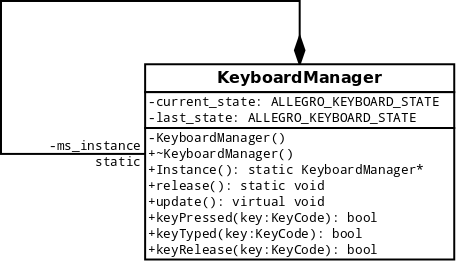
\includegraphics[scale = 0.4]{uml/KeyboardManager.png}
    \\Fonte: Elaborada pelos autores.
\end{figure}
%
%
\par
A classe KeyboardManager realiza o gerenciamento do teclado. A classe (Figura \ref{KeyboardManager}) possui duas variáveis do tipo ALLEGRO\_KEYBOARD\_STATE. Uma para guardar o último estado e outra para guardar o estado atual do teclado, de modo a conseguir verificar se determinada tecla foi pressionada, está sendo pressionada ou foi solta. Como o tipo ALLEGRO\_KEYBOARD\_STATE sugere, uma variável desse tipo armazena o estado (pressionada ou solta) de todas as teclas do teclado no momento em que o método \textit{update()} é chamado. Há outros três métodos que verificam se determinada tecla foi pressionada, continua pressionada ou se foi solta. Os métodos recebem como parâmetro o \textit{keycode} da tecla e retornam um tipo booleano. A seguir temos um exemplo de uso da classe KeyboardManager.
%
%
\begin{lstlisting}

  // Inicializamos os dispositivos de entrada
  KeyboardManager* keyboard = KeyboardManager::Instance();
  
  // Atualiza o estado das teclas
  keyboard->update();
	
  // Verifica se a seta direita esta pressionada
  if( keyboard->keyPressed( ALLEGRO_KEY_RIGHT ) ) {}
  
  // Verifica se a tecla ESC foi solta
  if( keyboard->keyRelease( ALLEGRO_KEY_ESCAPE ) ) {}
  
  // Verifica se a tecla SPACE foi pressionda
  if( keyboard->keyTyped( ALLEGRO_KEY_SPACE ) ) {}
	      
\end{lstlisting}
%
\subsection{MouseManager}
%
%
\begin{figure}[H]
    \centering
    \caption{UML detalhando a classe MouseManager.}
    \label{MouseManager}
    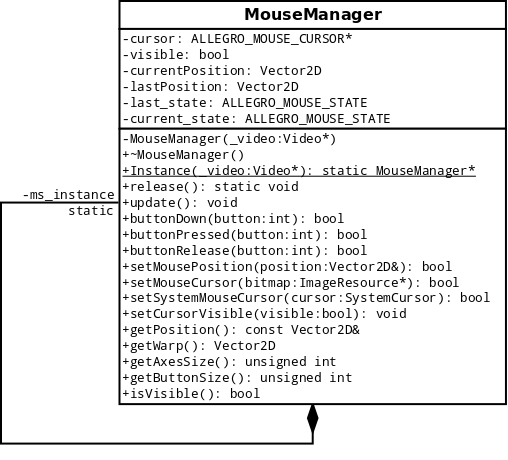
\includegraphics[scale = 0.40]{uml/MouseManager.png}
    \\Fonte: Elaborada pelos autores.
\end{figure}
%
%
\par
A classe MouseManager realiza o gerenciamento dos eventos gerados pelo \textit{mouse}. A classe (Figura \ref{MouseManager}) trabalha usando lógica semelhante a KeyboardManager, só que aplicada ao mouse. Ela Possibilita também deixar ou não visível o cursor do mouse na aplicação e alterar o estilo do cursor.
%
%
%=============================================================
\section{SGL Font}
%
%
É o pacote responsável pela parte textual da biblioteca. Ele carrega uma fonte no formato TTF (``True Type Font'') padrão do Windows e a utiliza para escrever um texto na tela.
%
%
%
\begin{figure}[H]
    \centering
    \caption{UML das classes FontResource e Font.}
    \label{Font}
    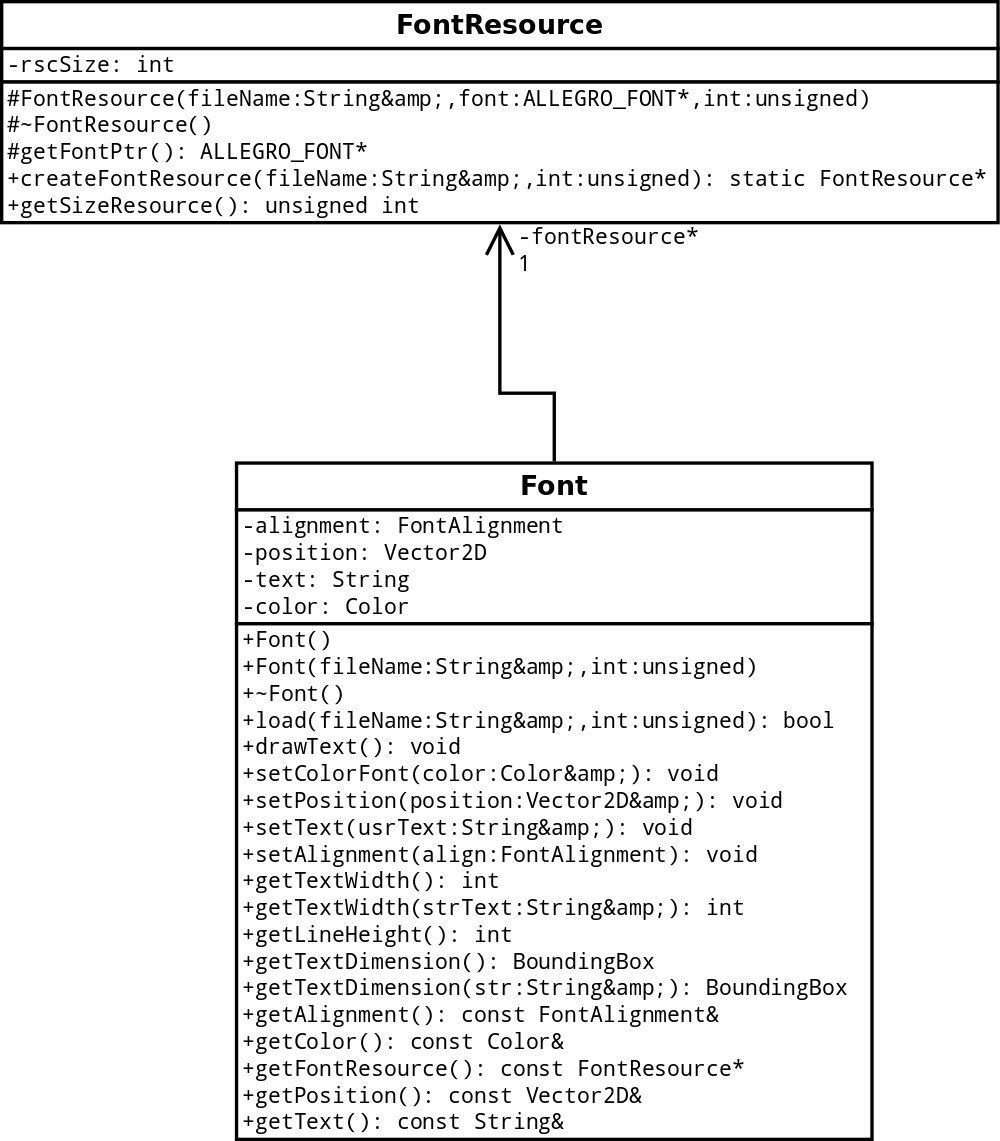
\includegraphics[scale = 0.20]{uml/Font.png}
    \\Fonte: Elaborada pelos autores.
\end{figure}
%
%
\subsection{FontResource}
%
%
A classe é uma especialização de Resource. Ela é usada dentro do método \textit{load()} da classe Font e funciona da seguinte maneira: recebe um arquivo TTF e o tamanho da fonte desejada, e em seguida esse arquivo é adicionado a uma instância da classe ResourceManager, caso ainda não tenha sido alocado. É possível existir dois arquivos de fonte iguais mas com tamanhos diferentes em ResourceManager, isso possibilita que utilizemos fontes iguais, mas com tamanho diferentes, uma medida necessária, uma vez que a Allegro não permite que alteremos o tamanho da fonte posteriormente.
%
%
\subsection{Font}
%
%
A classe Font (Figura \ref{Font}) possui métodos para escrever na tela e mudar as configurações do texto, tais como cor, alinhamento e posição. O pacote utiliza também as funcionalidades das classes Vector2D, Color e BoundingBox. Com os métodos \textit{gets} temos informações sobre as configurações atuais do objeto.
\par 
A seguir temos alguns exemplos de uso da classe. Para instanciar um objeto da classe Font utilizamos seu construtor, cujo primeiro parâmetro é o \textit{path} do arquivo TTF. A barra '/' indica hierarquia de diretórios a partir da pasta do projeto. Ou seja, dentro da pasta de projeto existe uma pasta chamada Resource e o arquivo alger.ttf se encontra nela. O segundo parâmetro é o tamanho da fonte.
%
\begin{lstlisting}
  // Criamos uma font
  Font alger("Resource/alger.ttf", 30);
\end{lstlisting}
%
\par
Alterando cor, alinhamento e posição. O tipo do alinhamento pode ser RIGHT, LEFT, CENTRE ou INTEGER.
%
\begin{lstlisting}
  // Definimos a cor da fonte
  alger.setColorFont(Color ("lightskyblue"));
  // Definimos seu alinhamento
  alger.setAlignment(FontAlignment::CENTRE);
  // Definimos sua posicao
  alger.setPosition(Vector2D(200, 100));
\end{lstlisting}
%
\par 
Definimos o texto que será exibido na tela e o escrevemos no \textit{display}:
%
\begin{lstlisting}
  // Definimos o texto a ser escrito no display
  alger.setText("Fonte: Alger");
  // Desenhamos o texto
  alger.drawText();
  // Definimos um novo texto para ser escrito
  alger.setText("Tamanho: 30");
  // Ajustamos a posicao do segundo texto
  alger.setPosition(Vector2D(200, 140));
  // Desenhamos o segundo texto na display
  alger.drawText();
  // Atualizamos o display
  video.refresh();
\end{lstlisting}
%
Após a execução do código acima, temos o seguinte texto no \textit{display} (Figura \ref{ExemploFont}).
%
%
%
\begin{figure}[H]
    \centering
    \caption{Exemplo de uso da classe Font.}
    \label{ExemploFont}
    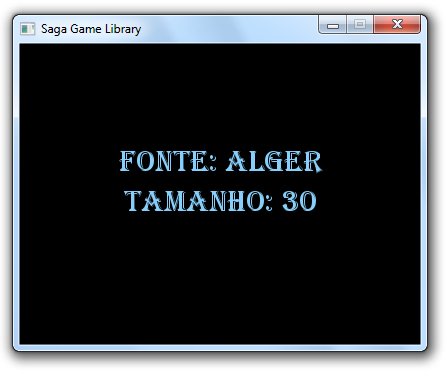
\includegraphics[scale = 0.70]{Imagens/ExemploFont.png}
    \\Fonte: Elaborada pelos autores.
\end{figure}
%
%
%
%=======================================================
\section{SGL Áudio}
%
%
É o pacote que realiza as funcionalidades referentes à parte sonora. É estruturado da seguinte maneira: de um lado a classe AudioResource, especialização de Resource, e da qual derivam AudioStreamResource e AudioSampleResource. Do outro lado, temos a classe abstrata Audio, da qual derivam AudioStream e AudioSample. As duas últimas relacionam-se com as respectivas especializações de AudioResource. Tal estrutura nos possibilita criar um objeto de AudioSample quando desejamos manipular um efeito sonoro, como um soco ou o barulho de uma explosão, ou um objeto de AudioStream quando precisamos usar uma trilha sonora.
\par 
AudioSample e AudioStream possuem em comum métodos para carregar, tocar, alterar ganho, balanço, velocidade e modo de repetição. Além desses, cada classe possui outros métodos com funções específicas. Entre os vários formatos de arquivos de áudio suportados, os mais usados são .wav e .ogg. Infelizmente não existe suporte ao formato MP3, por o mesmo se tratar de um formato de áudio proprietário (e também pouco usado em jogos).
\par
Exemplos:
\par 
Cria-se um objeto de  AudioSample, indicando o caminho onde o arquivo de áudio encontra-se.
%
\begin{lstlisting}
  // Criamos um sample
  AudioSample sample("Resource/audio/palmas.wav");
\end{lstlisting}
%
\par
Altera o ganho para 80\% do valor original e a velocidade para 90\% do valor original.
%
\begin{lstlisting}
  // Ajustamos o valor do ganho
  sample.setGain(0.8);
  // Ajustamos a velocidade de execucao do sample
  sample.setSpeed(0.9);
\end{lstlisting}
%
\par
Faz com que o arquivo continue tocando indefinidamente após chamar o método \textit{play()}.
%
\begin{lstlisting}
  // Ajustamos para reproducao em loop
  sample.setLoopingMode(AudioPlayMode::PLAY_LOOP);
\end{lstlisting}
%
\par
Finalmente, colocamos o arquivo para ser reproduzido.
%
\begin{lstlisting}
  // Iniciamos a reproducao do sample
  sample.play();
\end{lstlisting}
%
%
\par
O código a seguir carrega um arquivo para ser reproduzido como trilha sonora e recebe parâmetros para alterar o \textit{buffer} (em \textit{bytes}) e a taxa de amostragem.
%
\begin{lstlisting}
  // Carregamos um audiostream
  AudioStream stream("Resource/audio/interface.ogg", 4, 1024);
\end{lstlisting}
%
\par 
Inciamos a reprodução do o arquivo a partir dos 14 segundos.
%
\begin{lstlisting}
  // Definimos o tempo de inicio
  stream.setBegin(14);
  // Iniciamos a reproducao do audio stream
  stream.play();
\end{lstlisting}
%
%
%==============================================
%
\section{SGL Image}
%
Trata-se de um dos principais pacotes da \textit{SAGA Game Library}, contendo todas as classe referentes à manipulação de recursos de imagem. Apesar do pacote possuir um grande volume de classes, nos limitaremos às suas duas classes mais importantes: AnimatedSprite e TMXTileMap.
%
%
%
\subsection{TMXTileMap}
%
%
%
A grande maioria dos jogos eletrônicos 2D apresenta, além das imagens, também chamadas de \textit{sprites}, dos personagens e itens, uma imagem representando o cenário do jogo. Dependendo da natureza do jogo, esses cenários podem possuir grandes dimensões, o que torna custoso em termos computacionais armazenar essa imagem em memória (RAM e disco) e desenhá-la no \textit{display}. Entretanto, quando analisamos a imagem que representa o cenário, podemos verificar que o mesmo é formado por pequenas partes que se repetem com muita frequência. A definição formal do termo \textit{sprite} será mostrado na subseção sobre a classe AnimatedSprite.
\par
Assim, aproveitando dessa característica, com o objetivo de diminuir o consumo de memória e o desempenho na renderização e carregamento das imagens de resolução elevada, foi desenvolvida uma técnica conhecida como \textit{TileMap}, que consiste no uso de uma imagem, chamada \textit{tileset} (Figura \ref{tileset_edit}), contendo pequenos pedaços de imagens, conhecidos como \textit{tiles}, que são as imagens que se repetem em grande quantidade no cenário do jogo. Esses \textit{tiles} são usados para criar uma imagem composta denominada \textit{tiled layer} \cite{Novak}.
%
%
\begin{figure}[H]
    \centering
    \caption{Exemplo de \textit{tileset}.}
    \label{tileset_edit}
    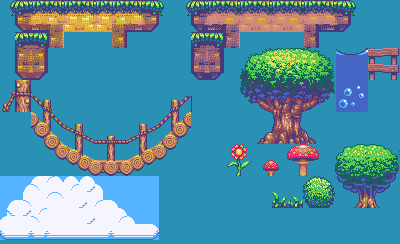
\includegraphics[scale = 1.0]{Imagens/tileset_edit.png}
    \\Fonte: \textit{Generic tileset} de autoria de Surt(OpenGameArt).
\end{figure}
%
\par
O cenário final do jogo (Figura \ref{cenario}) pode ser constituído de um único \textit{tiled layer} ou ser resultante da combinação de dois ou mais \textit{tiled layers}. Através da técnica de \textit{Tilemap}, torna-se possível construir inúmeros cenários, com variadas dimensões, usando como base o mesmo \textit{tilesets}, aumentando a economia de memória e não reduzindo o desempenho no carregamento de imagens.
%
%
%
\begin{figure}[H]
    \centering
    \caption{Exemplo de um cenário construído com \textit{tileset}.}
    \label{cenario}
    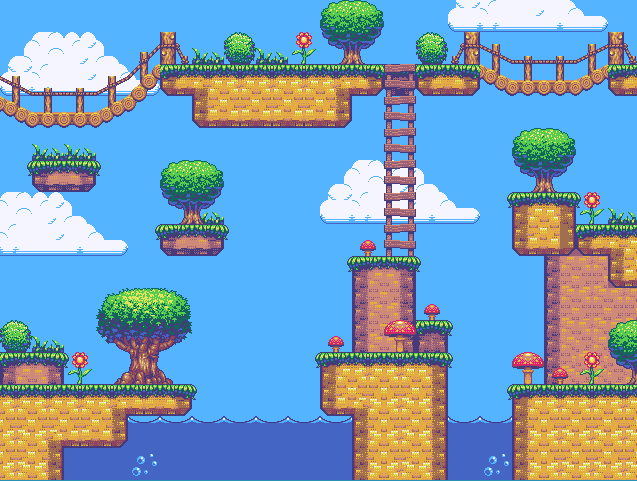
\includegraphics[scale = 0.65]{Imagens/cenario.png}
    \\Fonte: Elaborada pelos autores.
\end{figure}
%
%
%
%
\par 
A \textit{SAGA Game Library} também faz uso da técnica para criação de cenários e \textit{sprites} animados através do \textit{Tiled}. O Tiled nos fornece um arquivo XML personalizado chamado TMX, contendo todos os dados relevantes para a construção do cenário do jogo, e para ter acesso a esses dados torna-se necessário o uso de um \textit{parser} XML, para realizar a leitura do arquivo XML. O \textit{parser} escolhido foi a TinyXML, por sua baixa curva de aprendizado e velocidade de leitura. A seguir podemos visualizar um exemplo simples de um arquivo .tmx.
%
%
\lstinputlisting{CodigoFonte/novo.tmx}
%
\par 
Como pode ser observado, o arquivo .tmx possui todos os detalhes de cada \textit{tileset} usado na construção do cenário e os dados referentes a cada \textit{layer} criado. Uma das dificuldades de implementação do suporte ao Tiled foi desenvolver as rotinas de leitura desses dados, de modo a torná-las rápidas e de fácil uso. O resultado desse trabalho foi o desenvolvimento de classes responsáveis pela leitura de cada elemento do arquivo, de forma que cada um desses dados fosse armazenados em atributos para posteriormente serem usados pelo usuário. Assim foram implementadas as classe TMXTileSet e TMXLayer entre outras. Cada uma dessas classes é responsável por realizar o \textit{parsering} dos seus respectivos elementos e atributos (do arquivo .tmx). Por exemplo, a classe TMXLayer é responsável pela leitura dos elementos \textit{layer} e de seus respectivos atributos, \textit{name, width} e \textit{height} e também é responsável pela leitura, compressão (GZIP ou ZLIB) e decodificação (base64) usadas no elemento \textit{data}.
%
\par 
Quando observa-se o elemento \textit{data} do arquivo .tmx, verifica-se que ele possui dois atributos: \textit{encoding} e \textit{compression}. Esses atributos nos indicam se foi usada algum tipo de codificação (base64) e se algum algoritmo de compressão (GZIP ou ZLIB) foi aplicado. Para a descompressão foi utilizada a biblioteca ZLIB, que fornece métodos para se trabalhar com compressão usando GZIP e ZLIB, e para a decodificação foi usada o algoritmo desenvolvido por René Nyffenegger \footnote{http://www.adp-gmbh.ch/cpp/common/base64.html}, que fornece um modo muito prático de decodificação. Ambos os algoritmos, de compressão e descompressão funcionam da mesma maneira, é passada uma \textit{string} contendo os dados codificados/comprimidos e como retorno temos a \textit{string} decodificada/descomprimida. 
\par
Através dessa \textit{string}, nós criamos um vetor de inteiros (através da conversão de tipos) que contem os índices de cada \textit{tile} do \textit{tileset}. Feito isso, podemos desenhá-los, fazendo com que o nosso cenário criado seja visualizado no \textit{display}. Finalmente, a classe TMXTileMap contem os métodos para carregar e manipular os dados obtidos pela leitura do arquivo tmx, também provendo rotinas de verificação de colisão entre \textit{sprites}.
\par
Um cenário completo construído usando o \textit{software} pode ser visualizado na Figura \ref{snapshot1} e na Tabela \ref{TabelaTiled} é possível verificar a redução do tamanho em disco de um arquivo .tmx e do tempo de carregamento desse em relação ao tipo de codificação/compressão utilizada (quando utilizada). Através desses dados pode-se observar que o uso de codificação/compressão trouxe redução no tempo de carregamento do cenário.
%
%
\begin{figure}[ht]
    \centering
    \caption{Cenário construído usando o Tiled e a classe TMXTileMap.}
    \label{snapshot1}
    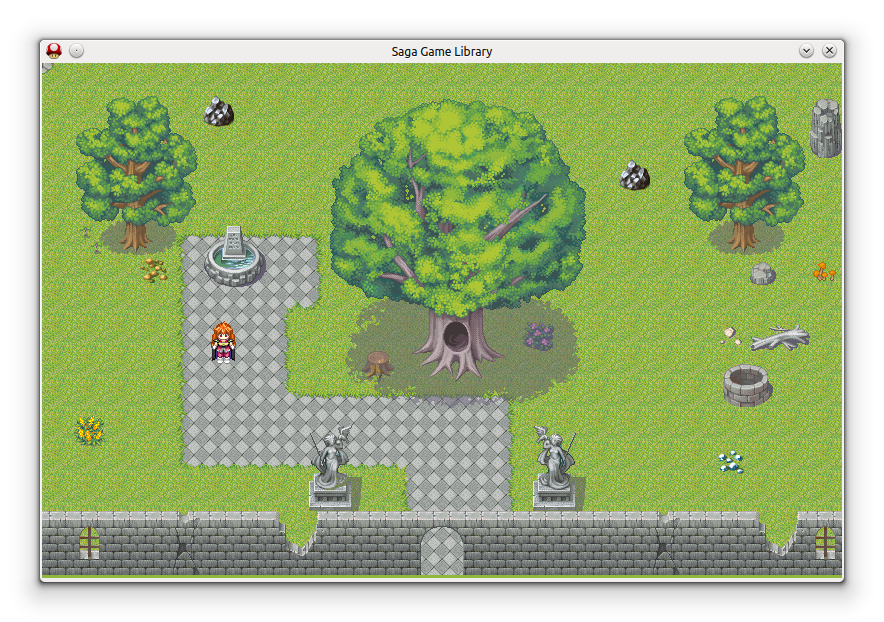
\includegraphics[scale = 0.60]{Imagens/snapshot1.png}
    \\Fonte: Elaborada pelos autores.
\end{figure}
%
%
\begin{table}[ht]
\centering
\caption{Comparação de tamanho em disco e tempo de carregamento do arquivo .tmx compactado/codificado.}
\label{TabelaTiled}
\begin{tabular}{|l|c|c|}\hline
\textbf{Codificação/Compressão} & \textbf{Tamanho em disco} & \textbf{Tempo de carregamento}\\\hline
\textbf{Apenas XML} & 31,3 KB & 0,10129 seg\\\hline
\textbf{Apenas Base 64} & 9,6 KB & 0,07337 seg\\\hline
\textbf{Base64 + ZLIB} & 2,1 KB & 0,07102 seg\\\hline
\textbf{Base64 + GZIP} & 2,2 KB & 0,07122 seg\\\hline
\textbf{CSV} & 4,9 KB & 0,07661 seg\\\hline
\end{tabular}
\\Fonte: Dados obtidos em simulações realizadas pelos alunos.
\end{table}
%
\par 
Como pode-se observar, o Tiled fornece grande comodidade no projeto de cenários. Pensando nisso, também foi adaptado o uso do Tiled para criarmos \textit{sprites} animados. As classes envolvidas são as mesmas usadas para se trabalhar com os cenários (com exceção da classe TMXTileMap).
%
%
\subsection{AnimatedSprite}
%
%
\textit{Sprites} são estruturas que permitem a criação de animações e permitem livre posicionamento na tela. De um modo geral, todas as imagens de um jogo podem ser denominadas \textit{sprites}. Um \textit{sprite} sempre possui um quadro fixo definido e pode ter vários conjuntos de animações configurados \cite{Novatec}. Os \textit{sprites} que possuem apenas uma quadro, ou seja, que não possuem animação são representados pela classe StaticSprite. Esta classe recebe um objeto ImageResource e o manipula, definindo sua posição no \textit{display}, realizando a renderização e verificando se ocorreu colisão desse com outro \textit{sprite}. Quanto à classe AnimatedSprite, ela apresenta funções muito mais complexas e interessantes, as quais serão abordadas a seguir.
\par 
A classe AnimatedSprite (Figura \ref{AnimatedSprite}) é usada quando se deseja ter um \textit{sprite} com suporte a animações. Essas animações são criadas através do Tiled, e carregadas posteriormente pelo método \textit{load()} da classe. Um objeto da classe AnimatedSprite é constituído de um vetor de objetos do Animation, que por sua vez possui uma coleção de objetos da classe Frame. Essas classes, como seus respectivos nomes sugerem, são responsáveis por armazenar os dados de cada animação criada para o \textit{sprite} animado.
%
%
%
\begin{figure}[H]
    \centering
    \caption{UML da classe AnimatedSprite e de suas classes auxiliares.}
    \label{AnimatedSprite}
    \includegraphics[scale = 0.40]{uml/AnimatedSprite.png}
    \\Fonte: Elaborada pelos autores.
\end{figure}
%
%
\par
A criação das animações faz uso de um \textit{tileset} chamado \textit{spritesheet} (Figura \ref{sprite}) que contem todas as imagens referentes às animações que o \textit{sprite} pode possuir. Cada animação possui um número de \textit{frames}, que são os quadros com o desenho do personagem em uma determinada posição \cite{GEDIGames}.
%
%
%
\begin{figure}[H]
    \centering
    \caption{Exemplo de \textit{spritesheet}.}
    \label{sprite}
    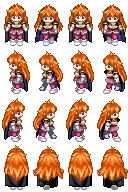
\includegraphics[scale = 1]{Imagens/sprite.png}
    \\Fonte: \textit{Spritesheet} de autoria de \cite{Sithjester}.
\end{figure}
%
%
%%
\par 
As animações são identificadas por \textit{labels} que são definidos durante a criação das animações com o Tiled e posteriormente podem ser acessadas com o método \textit{setCurrentAnimation()} da classe AnimatedSprite. O uso da AnimatedSprite proporciona grandes vantagens ao desenvolvedor ao oferecer suporte ao Tiled, tornando a criação de animações uma tarefa visual e mais atraente, fazendo uso do gerenciado de recursos ResourceManager para carregamento dos \textit{spritesheets} e possibilitando uso prático das animações. Vale ressaltar que a Allegro não possui suporte nativo à criação de \textit{sprites} animados, deixando o desenvolvedor responsável por implementar esse recurso. Felizmente, esse detalhe é contornado com o uso da AnimatedSprite, deixando o desenvolvedor livre para se focar em outras áreas mais importantes de seu projeto.
%
\par 
Para criarmos um \textit{sprite} animado usando a somente a Allegro, começamos definindo a estrutura de cada \textit{frame}.
%
\begin{lstlisting}
  /* Constantes do sprite */
  const int MAX_FRAMES  = 12;
  const int NUM_COLUNAS = 5;
  const int NUM_LINHAS  = 3;
  
  /* Definimos as propriedades do sprite */
  typedef struct Sprite
  {
      // Recebe o bitmap do sprite
      ALLEGRO_BITMAP* vetorSprites[ MAX_FRAMES ];
      // Guarda posicao dos sprites
      float pos_x, pos_y;
  } Sprite;
\end{lstlisting}
%
Em seguida criamos um \textit{sprite} que possui apenas uma animação. Essa animação funciona em \textit{loop}, ou seja, quando o último \textit{frame} da animação for desenhado, a animação volta a se repetir desde o primeiro \textit{frame}.
%
\lstinputlisting{CodigoFonte/SpriteExemplo.cpp}
%
\par 
A seguir, temos a criação de um \textit{sprite} animado usando a classe AnimatedSprite, considerando que já temos o arquivo .tmx com todas as animações prontas.
%
\lstinputlisting{CodigoFonte/ExemploAnimatedSprite.cpp}
%
Com o código acima, fica evidente a vantagem de usar a AnimatedSprite para criar \textit{sprites} animados ao invés de utilizar a apenas a Allegro.
%
%
%
\section{Testes}
%
A fase de testes consistiu simplesmente no uso das classes implementadas buscando erros de execução e \textit{bugs}. Não foi utilizada nenhuma ferramenta específica para testes de \textit{software}, devido à pouca experiência da equipe com essas ferramentas, ao tempo disponível para terminar essa versão do projeto e também à constatação das vantagens da \textit{SAGA Game Library}, não só na performance, mas também na usabilidade. Muitos dos resultados dos testes foram descritos nesse relatório, como as medições de consumo de memória e o tempo de carregamento da classe ResourceManager. 
%

